\section{Data used for Validation}
\label{validation:data}

\subsection{Consumers}

This work considers real-world demand data of energy consumers.
It takes the data from two different sources.
\begin{enumerate*}
  \item Smart meters that Georgievski et al. \cite{Georgievski2012} installed in an office.
  \item Adaptive Charging Network (ACN) electric vehicle charging stations at the Californian Institute of Technology. \cite{Lee2019, ACNCaltech2020}
\end{enumerate*}

The data from the smart meters spans about $8$ months.
It is from the year 2016.
It has a time resolution of $10$ seconds.
The program transforms the data to have a time resolution of $10$ minutes.
It does so by adding up the energy demand of $10$ minute periods and then dividing by $0.166$ hours since the data is given as energy in kWh.
The result is the power given in kW.

The data from the ACN charging stations spans the first $9$ months of the year 2020.
It consists of various charging sessions.
The program identifies the energy demand by assuming the charger transfers energy to the car at one fixed rate in one session.
This is not the point of adaptive charging, but it gives a real-world-like representation of electric vehicle charging behavior.
The time resolution of the resulting data is $10$ minutes.

The program computes the average day of both datasets.
Then it combines both datasets.
The data from the smart meters is weighted $1, 000 : 1$ against the data from the ACN charging stations.
This composition is due to the low energy demand of one office.
The final data represents an average day of one electric vehicle charging site and $1, 000$ offices with a $10$ minute time resolution.
It is shown in figure \ref{figure:data.demand.day}.

\begin{figure}
  \centering
  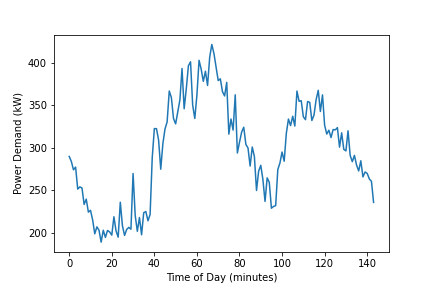
\includegraphics[width=0.7 \textwidth]{04_Validation/data_demand_day.png}
  \caption{Demand Data}
  \label{figure:data.demand.day}
\end{figure}

\subsection{Producers}

\todo{List data of plants}
